% Options for packages loaded elsewhere
\PassOptionsToPackage{unicode}{hyperref}
\PassOptionsToPackage{hyphens}{url}
%
\documentclass[a4paper,12pt
]{article}
\usepackage{times,fullpage,polski}
\usepackage{amssymb,amsmath}
\usepackage{ifxetex,ifluatex}
\ifnum 0\ifxetex 1\fi\ifluatex 1\fi=0 % if pdftex
  \usepackage[T1]{fontenc}
  \usepackage[utf8]{inputenc}
  \usepackage{textcomp} % provide euro and other symbols
\else % if luatex or xetex
  \usepackage{unicode-math}
  \defaultfontfeatures{Scale=MatchLowercase}
  \defaultfontfeatures[\rmfamily]{Ligatures=TeX,Scale=1}
\fi
% Use upquote if available, for straight quotes in verbatim environments
\IfFileExists{upquote.sty}{\usepackage{upquote}}{}
\IfFileExists{microtype.sty}{% use microtype if available
  \usepackage[]{microtype}
  \UseMicrotypeSet[protrusion]{basicmath} % disable protrusion for tt fonts
}{}
\makeatletter
\@ifundefined{KOMAClassName}{% if non-KOMA class
  \IfFileExists{parskip.sty}{%
    \usepackage{parskip}
  }{% else
    \setlength{\parindent}{0pt}
    \setlength{\parskip}{6pt plus 2pt minus 1pt}}
}{% if KOMA class
  \KOMAoptions{parskip=half}}
\makeatother
\usepackage{xcolor}
\IfFileExists{xurl.sty}{\usepackage{xurl}}{} % add URL line breaks if available
\IfFileExists{bookmark.sty}{\usepackage{bookmark}}{\usepackage{hyperref}}
\hypersetup{
  hidelinks,
  pdfcreator={LaTeX via pandoc}}
\urlstyle{same} % disable monospaced font for URLs
\usepackage{graphicx}
\makeatletter
\def\maxwidth{\ifdim\Gin@nat@width>\linewidth\linewidth\else\Gin@nat@width\fi}
\def\maxheight{\ifdim\Gin@nat@height>\textheight\textheight\else\Gin@nat@height\fi}
\makeatother
% Scale images if necessary, so that they will not overflow the page
% margins by default, and it is still possible to overwrite the defaults
% using explicit options in \includegraphics[width, height, ...]{}
\setkeys{Gin}{width=\maxwidth,height=\maxheight,keepaspectratio}
% Set default figure placement to htbp
\makeatletter
\def\fps@figure{htbp}
\makeatother
\setlength{\emergencystretch}{3em} % prevent overfull lines
\providecommand{\tightlist}{%
  \setlength{\itemsep}{0pt}\setlength{\parskip}{0pt}}
\setcounter{secnumdepth}{-\maxdimen} % remove section numbering



\begin{document}


\title{Rozwiązania chmurowe dla obliczeń
kwantowych\\ {\normalsize Stan na październik
2022}}

\author{Jarosław Miszczak}
\date{16/10/2022}

\maketitle

\begin{abstract}
Raport przedstawia zestawienie systemów udostępniających możliwość
wykonywania obliczeń kwantowych z poziomu chmury obliczeniowej.
Uwzględnione są rozwiązania poszczególnych firmy produkujących komputery
kwantowe jak rozwiązania dostawców usług obliczeniowych.
\end{abstract}



\hypertarget{amazon-braket}{%
\subsubsection{Amazon Braket}\label{amazon-braket}}

Amazon Braket to w pełni zarządzana usługa obliczeń kwantowych, która ma
pomóc w przyspieszeniu badań naukowych i rozwoju oprogramowania dla
obliczeń kwantowych. Usługa pozwala na zapoznanie się z możliwościami
programowania komputerów kwantowych i zbadać potencjalne zastosowania.
Amazon Braket zapewnia środowisko programistyczne, który można uruchomić
lokalnie na laptopie lub w pełni zarządzanym środowisku notebooków w
chmurze obliczeniowej.

\begin{figure}
\centering
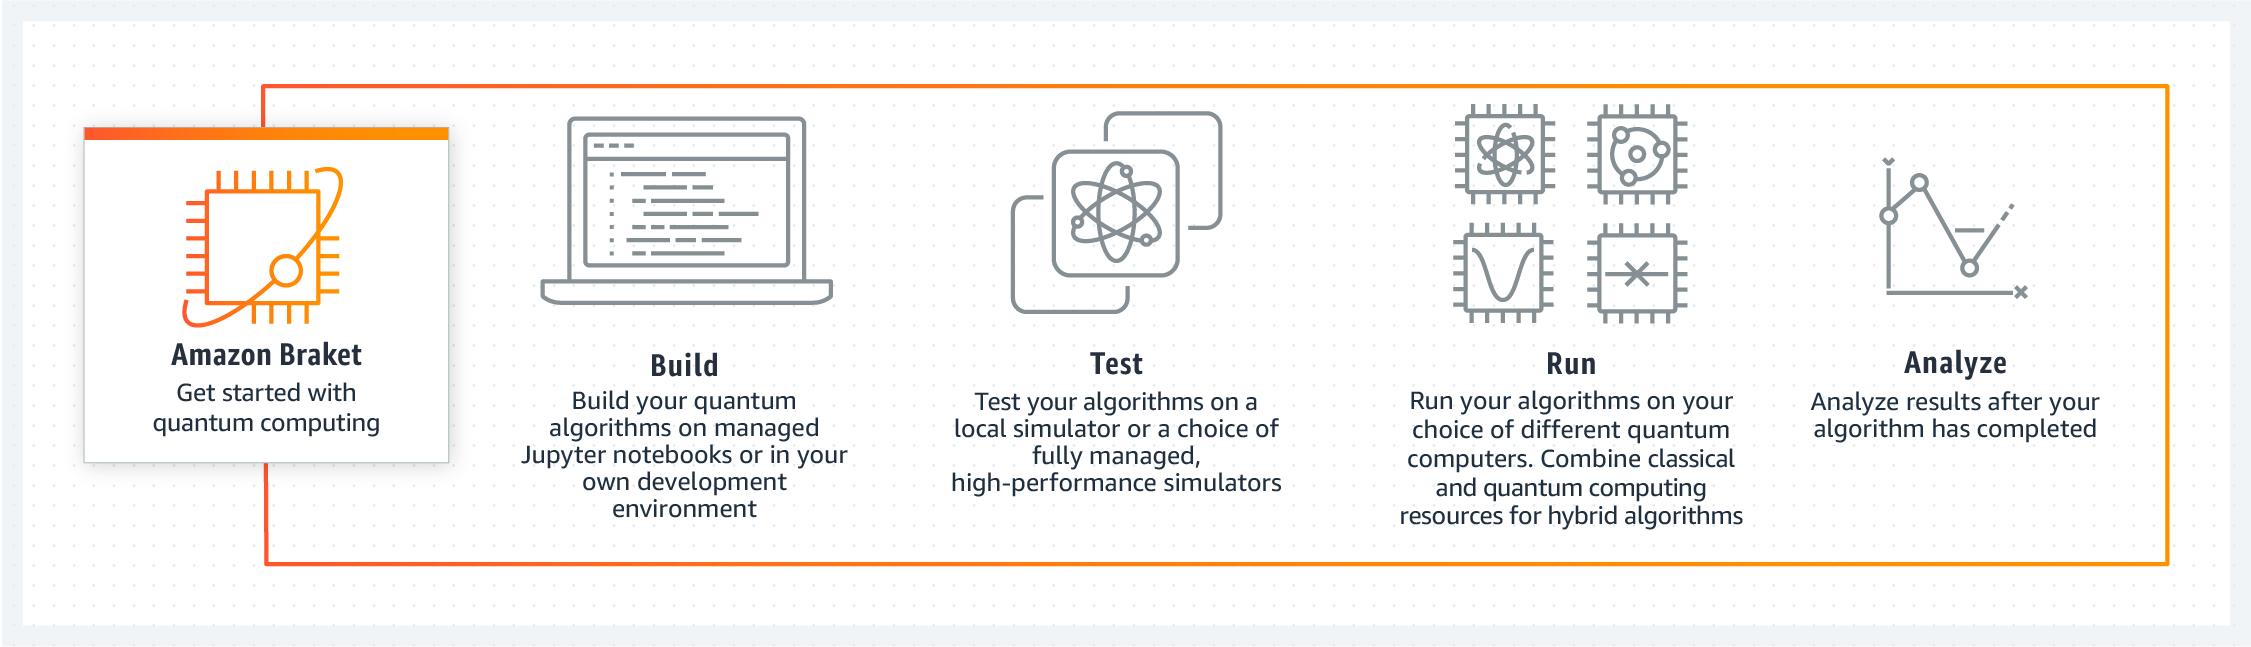
\includegraphics{amazon-braket-diagram.png}
\caption{Koncepcja funkcjonowania dostępu do maszyn kwantwoych w
serwisie Amazon Braket}
\end{figure}

W chwili obecnej Amazon Braket udostępnia urządzenia firm D-Wave, ION Q,
Oxford Quantum Circuit, Rigetti oraz Xanadu. Każde z tych urządzeń jest
zbudowane w opariu o innny zestaw technologi i możliwości programowania.

\begin{figure}
\centering
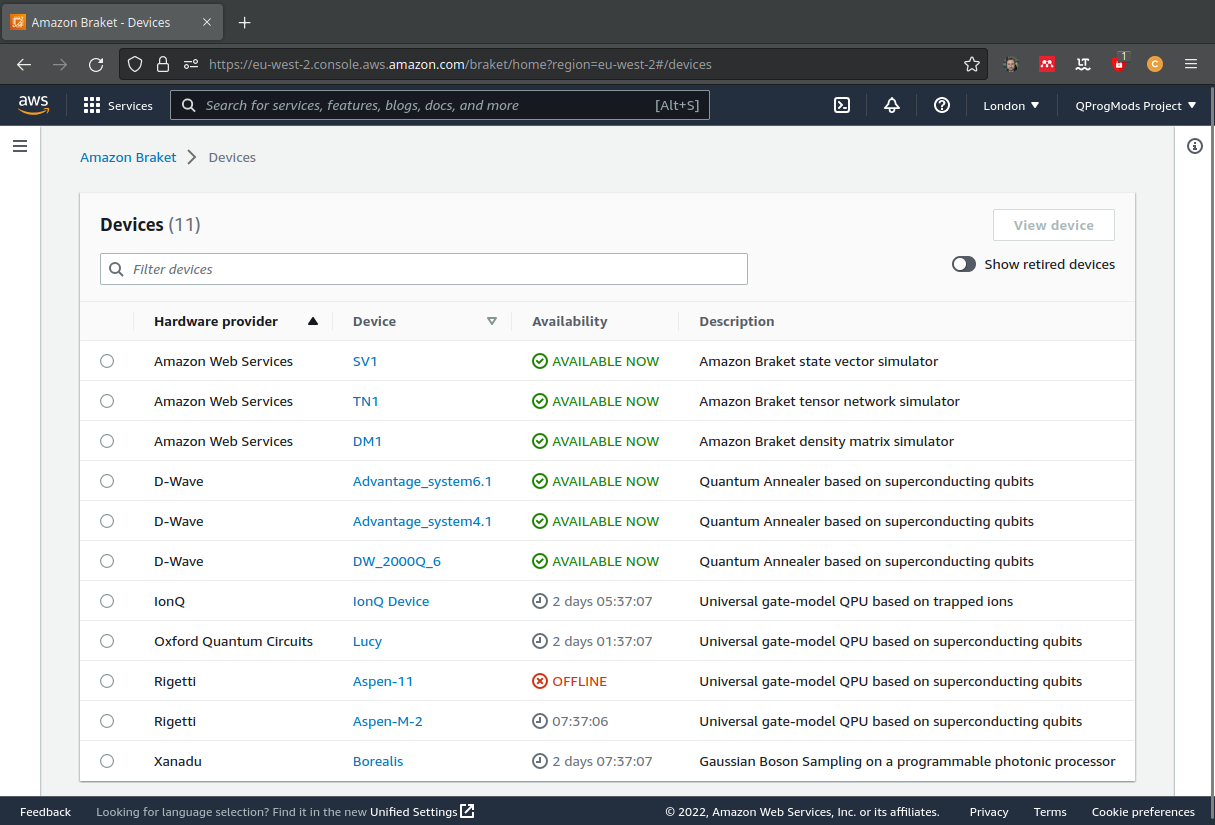
\includegraphics{amazon-braket-10.0222.png}
\caption{Urządzenia kwantowe dostępne poprzed interfejs AWS. Stan na
październik 2022}
\end{figure}

\hypertarget{google-cloud-platfrom}{%
\subsubsection{Google Cloud Platfrom}\label{google-cloud-platfrom}}

Google Cloud oferuje dostęp do komputera firmy IonQ w ramach usłudi
zarządzanej. Udsotępniana maszyna pozwala na wykonywania obliczeń z
pamięcią kwantową 11 kubitów.

\begin{figure}
\centering
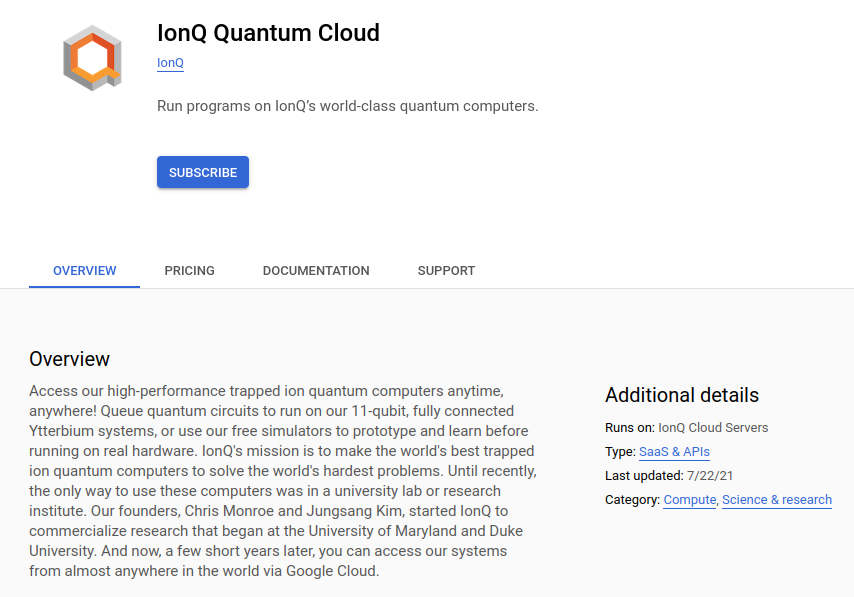
\includegraphics{google-cloud-ionq-10.2022.png}
\caption{Informacje o usłudzie dostępu do komputera IonQ z poziomu
Google Cloud console}
\end{figure}

Usługi zarządzane są w pełni hostowane, zarządzane i obsługiwane przez
usługodawców. Aby korzystać z usługi konieczna jest rejstracja się u
usługodawcy. Natomiast firma Google zajmuje się rozliczeniami kosztów
korzystania ze sprzętu.

Usługa ta jest dostępna poprzez wybranie jej z usług Google Cloud
Marketplace.

\hypertarget{xanadu-cloud}{%
\subsubsection{Xanadu Cloud}\label{xanadu-cloud}}

Firma Xanadu udostępniła swój komputer w czerwcu 2022. Udostępniony
komputer to Borealis, programowalny fotoniczny komputer kwantowy z 216
qubitami w stanie ściśniętym. MAszyn ta zostałą wykorzystana do
uzyskania czyli który przewyższa najlepsze klasyczne superkomputery w
konkretnym zadaniu, dostępny dla ludzi wszędzie poprzez Xanadu Cloud i
Amazon Braket.

\begin{figure}
\centering
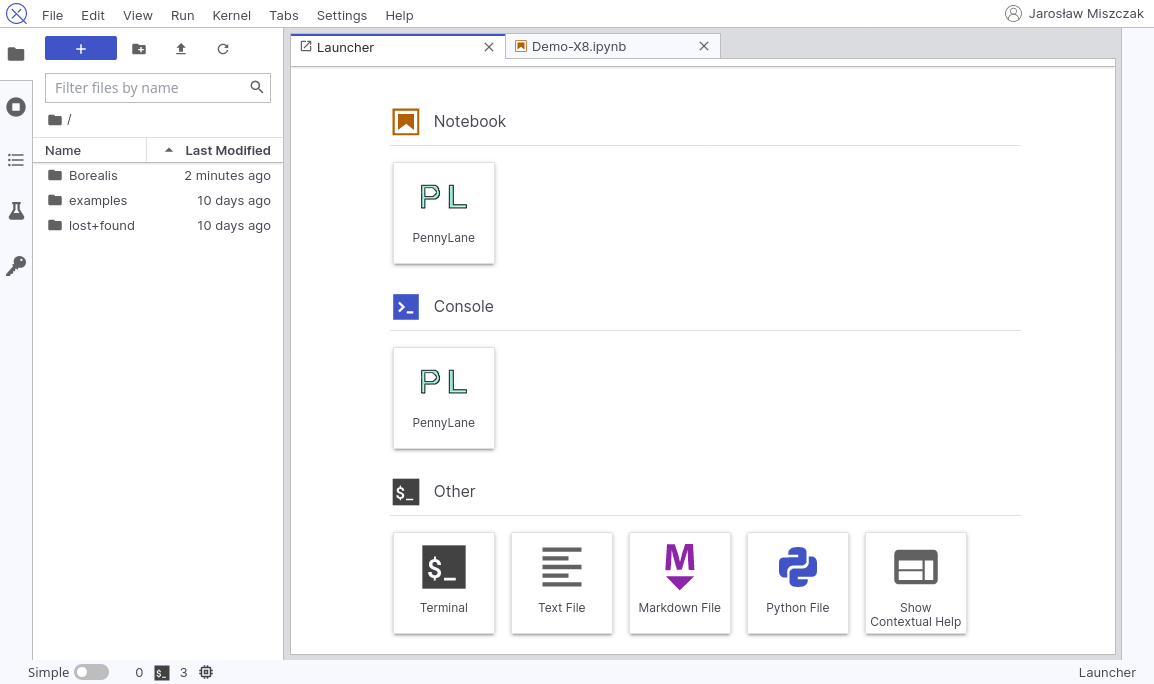
\includegraphics{xanadu-cloud-interface.png}
\caption{Interfejs użytkownika udostępniany w Xandau Cloud}
\end{figure}

Xanadau Cloud dostarcza interfejsu opratego o Jupyter Lab. Firma
dostarcza również zestawy przykładów oraz tutoriali pozwalających na
zaznajomienie się z proramowaniem w bibliotece PennyLane.

\hypertarget{ibm-qunatum}{%
\subsubsection{IBM Qunatum}\label{ibm-qunatum}}

IBM Quantum Composer i IBM Quantum Lab tworzą platformę internetową
umożliwiającą publiczny i premium dostęp do opartych na chmurze usług
obliczeń kwantowych świadczonych przez IBM Quantum. Obejmuje to dostęp
do zestawu prototypowych procesorów kwantowych IBM, zestawu samouczków
dotyczących obliczeń kwantowych oraz dostęp do interaktywnego
podręcznika.

\begin{figure}
\centering
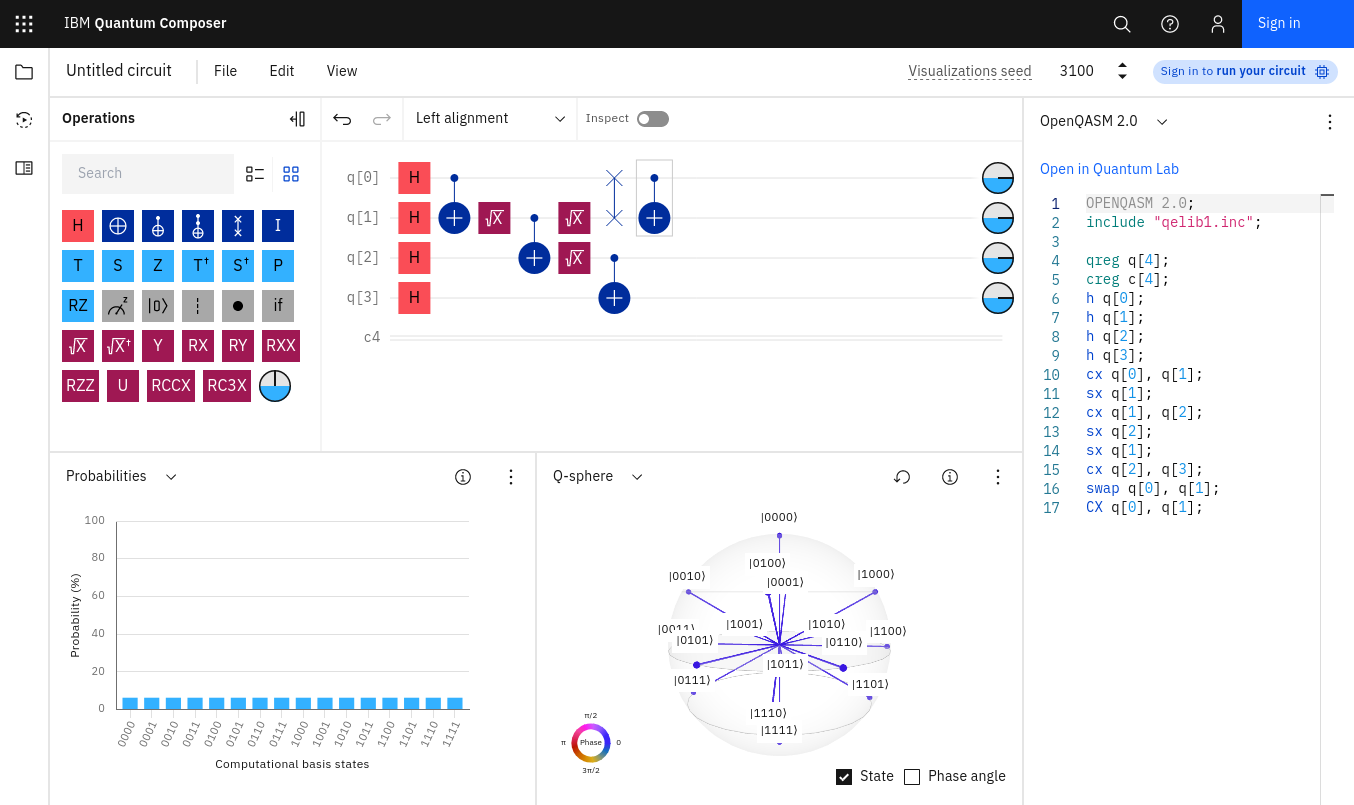
\includegraphics{ibm-q-composer.png}
\caption{Przykład wykorzystania narzędzia Composer w systemie IBM
Quantum}
\end{figure}

IBM Quantum pozwala również na zarządzania zasobami komputerowymi
przypisanymi do danego konta. W tej chili w podstawowoje wersji
dostępnych jest sześć komputerów o maksymalnej pamięci 7 qubitów. IBM
udostępnia równiez spejalizowane symulatory pozwalające na testowanie
kodu kwantowego w różnych scenariuszach.

\begin{figure}
\centering
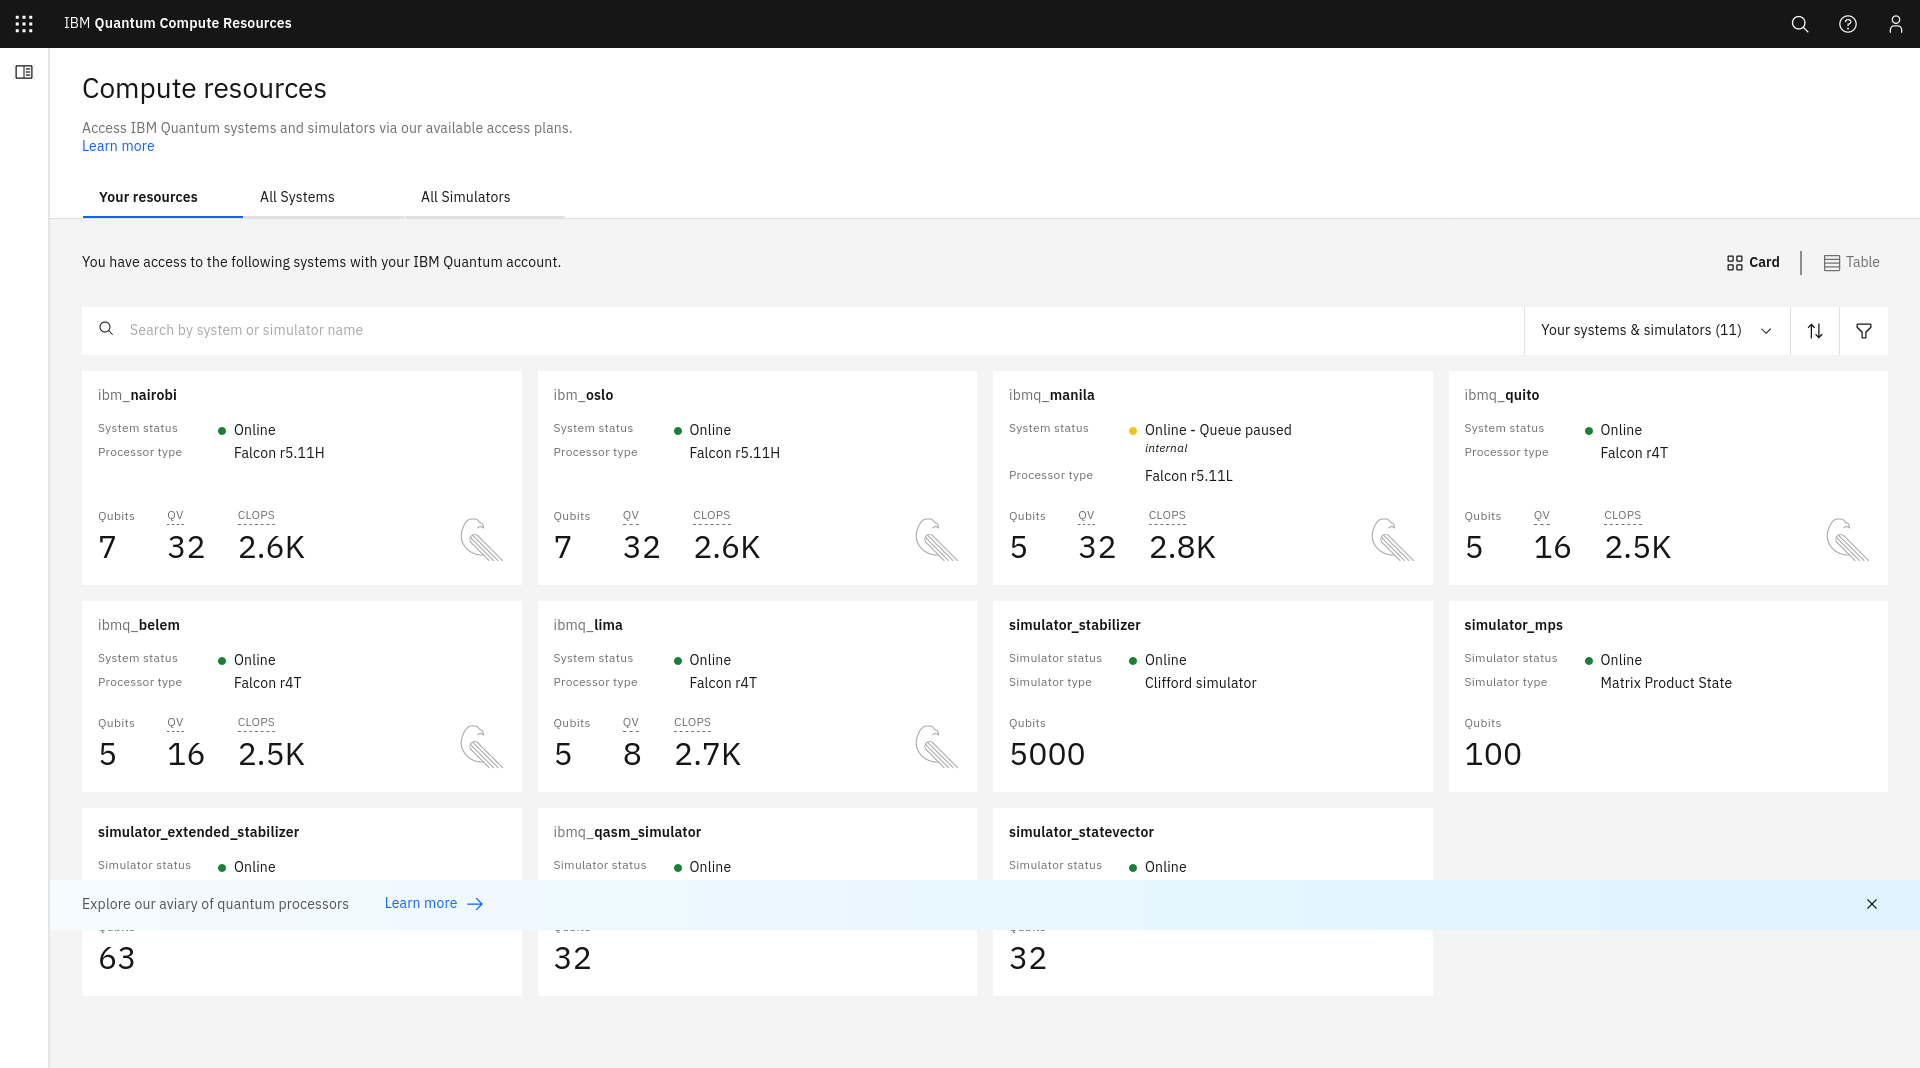
\includegraphics{ibm-q-resources.png}
\caption{Zarządzanie zasobami komputerowymi w paneu IBM Quantum}
\end{figure}

\hypertarget{d-wave-systems}{%
\subsubsection{D-Wave Systems}\label{d-wave-systems}}

Oprogramowanie Ocean to pakiet narzędzi, które D-Wave Systems udostępnia
na repozytorium D-Wave GitHub do rozwiązywania trudnych problemów z
wykorzystaniem komputerów kwantowych.

Dostęp do wyżażacza D-Wave systems jest możliwy poprzez interfejst Leap.
Interfejs ten zapewnie kontrolę na wykorzystaniem zasobó obliczniowych.
Dostarcza również środowiska progrmistycznego bazującego na VS Code oraz
zintegrowanego z GitHub i GitPod.

\begin{figure}
\centering
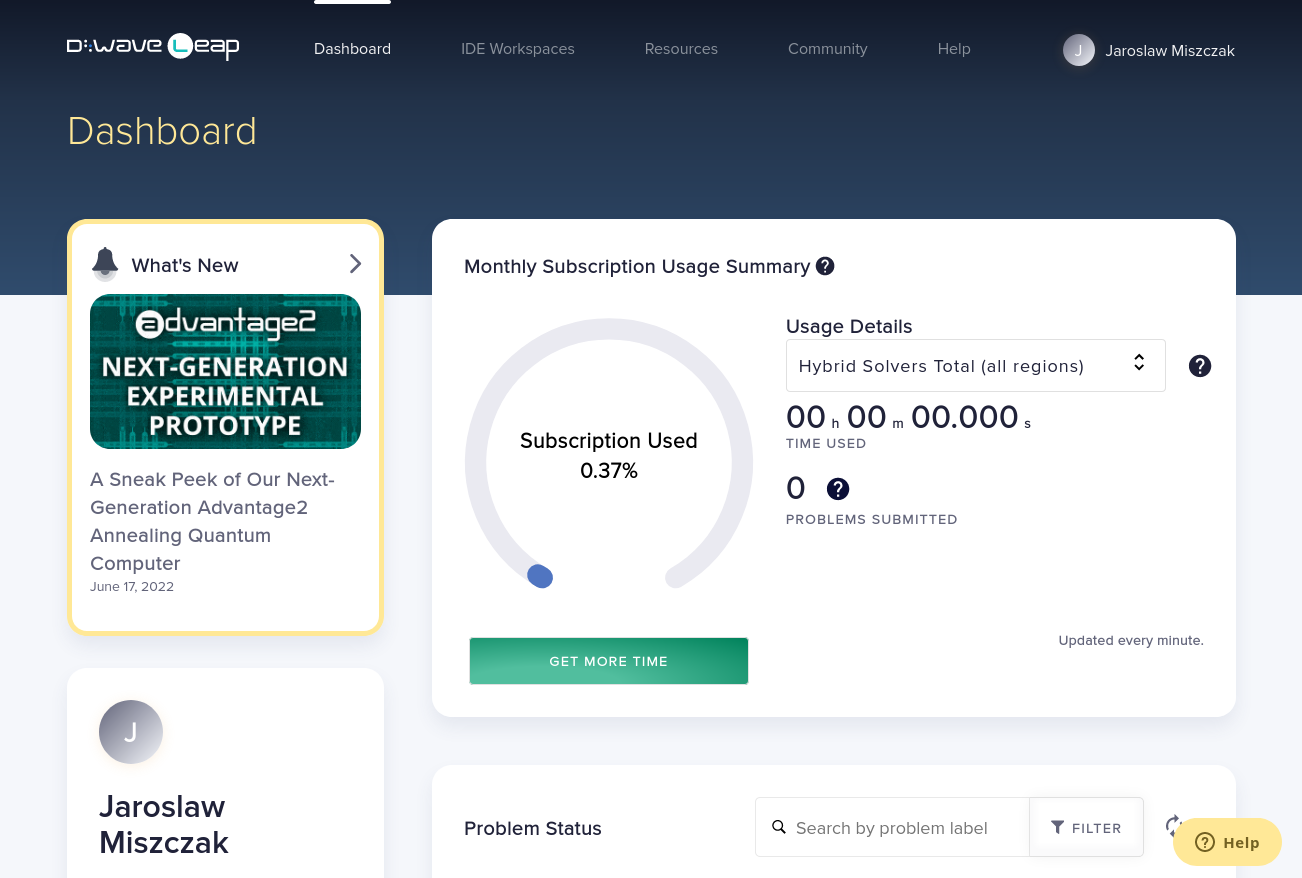
\includegraphics{d-wave-leap-dashboard.png}
\caption{Widok zarządzania wykorzystaniem czasu obliczeniowego w
systemie D-Wave Leap.}
\end{figure}

\hypertarget{ionq}{%
\subsubsection{IONQ}\label{ionq}}

Firma IonQ, opróc dostępu poprzez Google Cloiud Platfrom, udostępnia
również narzędzie do kontrolowania kolejki wykonania peocesów na
maszynie waktowej.

Dodatkowo, możliwe jest uruchamianie zadań na komputerze IonQ z poziomu
biblioteki Qiskit.

\hypertarget{aqt}{%
\subsubsection{AQT}\label{aqt}}

Firma AQT udostępnia w tej chili symulator pułpki jonowej. Obecnie
dostępne są idealne i zaszumione symulatory do uruchamiania obwodów
kwantowych. Trwają prace nad udostępnieniem sprzętu kwantowego.

\begin{figure}
\centering
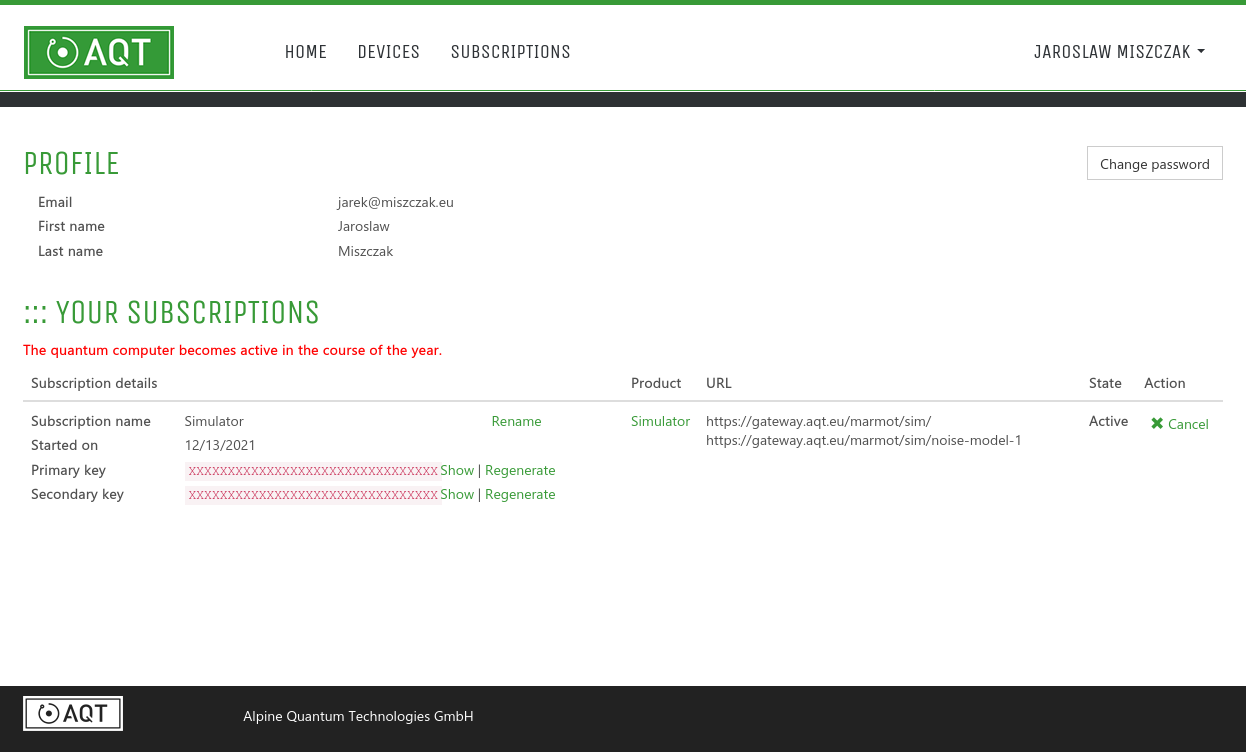
\includegraphics{aqt-subscriptions.png}
\caption{Zarządzanie subskrypcją z poziomu interfejsu firmy AQT}
\end{figure}

\hypertarget{ux17aruxf3dux142a}{%
\paragraph{Źródła}\label{ux17aruxf3dux142a}}

\begin{enumerate}
\def\labelenumi{\arabic{enumi}.}
\tightlist
\item
  https://www.aboutamazon.com/news/aws/aws-launches-new-quantum-computing-center,
  October 28, 2021
\item
  https://aws.amazon.com/braket/
\item
  https://cloud.google.com/blog/products/compute/ionq-quantum-computer-available-through-google-cloud,
  June 18, 2021
\item
  https://cloud.xanadu.ai/
\item
  https://www.xanadu.ai/press/xanadu-launches-first-public-cloud-deployed-computer-with-quantum-computational-advantage,
  June 1, 2022
\item
  L.S. Madse, et al., Quantum computational advantage with a
  programmable photonic processor, Nature, 606, pages 75--81 (2022),
  https://doi.org/10.1038/s41586-022-04725-x
\item
  https://pennylane.ai/
\item
  https://cloud.dwavesys.com/leap/
\item
  https://www.gitpod.io/
\item
  https://www.ibm.com/quantum
\item
  https://quantum-computing.ibm.com
\item
  https://cloud.ionq.com
\item
  https://gateway-portal.aqt.eu/
\end{enumerate}

\end{document}
